\chapter{Theory and Fundamentals of Project}

Developing an intelligent framework for Trade-Based Money Laundering detection requires a strong foundation in financial crime analysis, graph theory, and machine learning techniques. This chapter presents the fundamental concepts associated with Trade-Based Money Laundering, Graph Neural Networks, Graph Attention mechanisms, heterogeneous graph representation, and federated learning. The chapter further discusses the computational principles involved in relational transaction modeling, privacy-preserving learning, and real-time fraud analytics. These concepts collectively form the theoretical foundation for the proposed fraud detection framework.

%========================================================
\section[Trade-Based Money Laundering ]{\textbf{Trade-Based Money Laundering }}
%========================================================

\gls{tbml} is a sophisticated form of financial crime in which illicit funds are transferred and concealed through seemingly legitimate international trade activities. Unlike conventional laundering methods that primarily depend on direct financial transactions, TBML exploits import-export systems, trade invoices, shipping documents, and cross-border commercial operations to disguise the movement of illegal funds. Due to the increasing implementation of strict \gls{aml} regulations and \gls{kyc} policies, criminal organizations have increasingly shifted toward trade-oriented laundering mechanisms that are comparatively difficult to detect using traditional monitoring systems.

The complexity of modern global trade ecosystems, combined with the involvement of multiple financial entities and transactional relationships, has made TBML detection a major challenge for financial institutions and regulatory agencies. Consequently, intelligent analytical techniques capable of identifying hidden transactional dependencies and suspicious financial behavior have become increasingly important in modern Anti-Money Laundering systems.

%========================================================
\subsection[Introduction to TBML]{\textbf{Introduction to TBML}}
%========================================================

Trade-Based Money Laundering primarily involves the manipulation of international trade transactions to illegally transfer value between entities located across different countries. Criminal organizations often misuse trade documentation, invoice values, shipment quantities, and commercial agreements to move illicit funds while making the transactions appear legitimate within global financial systems. Since these laundering activities are embedded within regular import-export operations, identifying suspicious behavior becomes highly challenging for financial institutions and regulatory agencies.

In many TBML operations, colluding buyers and sellers intentionally manipulate the declared value of traded goods to transfer illegal financial assets across borders. Techniques such as over invoicing, under invoicing, phantom shipments, and multiple invoicing are commonly used to conceal the movement of illicit proceeds. Such laundering mechanisms exploit the complexity and high transactional volume of international trade systems, making traditional rule-based Anti-Money Laundering approaches comparatively ineffective in detecting hidden financial relationships.

\vspace{0.4cm}
\begin{figure}[H]
\centering
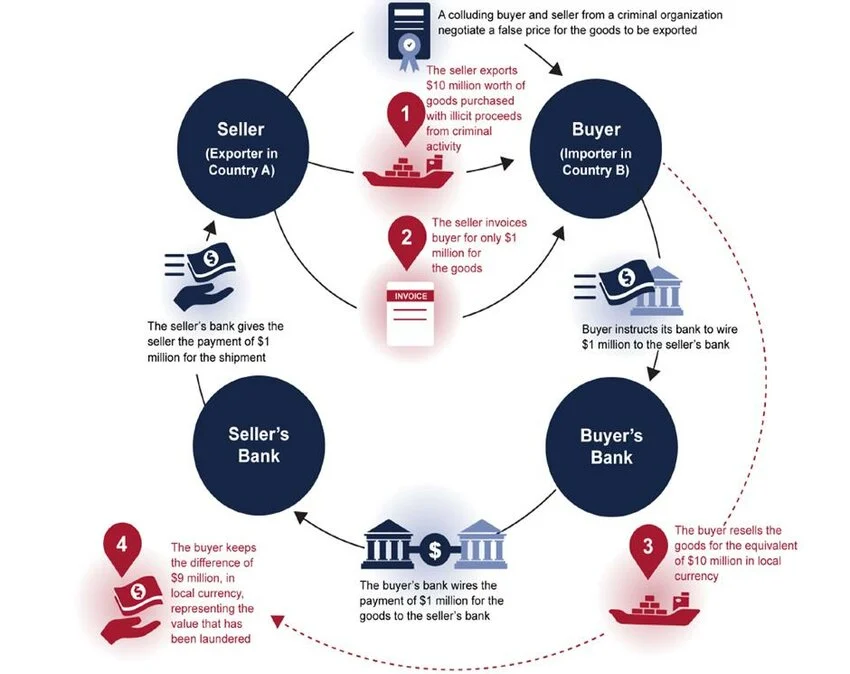
\includegraphics[width=0.82\textwidth]{./Figures/tbmlcycle.png}

\caption{Trade-Based Money Laundering through trade misinvoicing and open-account transactions}
\label{fig:tbml_cycle}

\end{figure}

\vspace{-0.2cm}

\noindent
\textit{Source: Adapted from ``The Role of Misinvoicing in the Money Laundering Cycle,'' 
\href{https://www.researchgate.net/figure/TBML-through-Open-Account-Transactions_fig1_370021180}{ResearchGate}.}

\vspace{0.3cm}

Figure~\ref{fig:tbml_cycle} illustrates a typical Trade-Based Money Laundering workflow involving collusion between exporters and importers across different jurisdictions.

%========================================================
\subsection[Common Techniques Used in TBML]{\textbf{Common Techniques Used in TBML}}
%========================================================

Trade-Based Money Laundering activities are generally performed through the manipulation of trade documentation, shipment details, pricing structures, and financial transactions associated with international trade operations. Criminal organizations exploit the complexity of global trade ecosystems to transfer illicit value across borders while making the transactions appear legitimate. Several laundering techniques are commonly used within modern trade systems to disguise the movement of illegal funds and avoid detection from financial monitoring authorities.

%========================================================
\subsubsection[Over Invoicing]{\textbf{Over Invoicing}}
%========================================================

Over invoicing is a laundering technique in which the value of exported or imported goods is intentionally declared higher than the actual market value. In this process, the buyer transfers an inflated payment amount to the seller, allowing excess funds to be moved across borders under the appearance of legitimate trade transactions. Criminal organizations use this technique to transfer illicit financial assets while avoiding suspicion from conventional banking systems.

%========================================================
\subsubsection[Under Invoicing]{\textbf{Under Invoicing}}
%========================================================

Under invoicing involves declaring a lower value for traded goods when compared to their actual market price. This technique allows the buyer or seller to secretly transfer additional financial value outside formal banking channels. Under invoicing is commonly used to evade taxes, conceal illegal profits, and facilitate hidden movement of illicit assets across jurisdictions.

%========================================================
\subsubsection[Multiple Invoicing]{\textbf{Multiple Invoicing}}
%========================================================

Multiple invoicing refers to the repeated use of the same trade invoice to justify several financial transactions for a single shipment of goods. By duplicating invoices across multiple banking channels or financial institutions, criminal entities can move large amounts of illicit funds while creating the appearance of legitimate trade payments. Detecting such duplicated transactional behavior is challenging in traditional rule-based monitoring systems.

%========================================================
\subsubsection[Phantom Shipments]{\textbf{Phantom Shipments}}
%========================================================

Phantom shipment laundering occurs when financial transactions are conducted for goods that are never actually shipped or delivered. Fraudulent trade documentation and fabricated shipping records are used to create the illusion of legitimate trade activity while transferring illicit funds between colluding entities. Since no physical goods are exchanged, identifying phantom shipment activities requires strong transactional verification and relational analysis mechanisms.

%========================================================
\subsubsection[Misrepresentation of Goods]{\textbf{Misrepresentation of Goods}}
%========================================================

Misrepresentation of goods involves intentionally providing false descriptions regarding the type, quantity, quality, or category of traded products within commercial documents and invoices. Criminal organizations use this technique to manipulate trade valuations and conceal suspicious financial activities under legitimate business transactions. Such inconsistencies are difficult to identify using isolated transactional analysis methods due to the large volume and diversity of international trade operations.

%========================================================
\subsection[Challenges in Detecting TBML]{\textbf{Challenges in Detecting TBML}}
%========================================================

Detecting \gls{tbml} activities is highly challenging due to the complexity and interconnected nature of modern international trade ecosystems. Unlike conventional financial fraud, TBML transactions are often embedded within legitimate commercial operations, making suspicious activities difficult to distinguish from regular trade behavior. Criminal organizations exploit multiple jurisdictions, shell companies, intermediaries, and layered transactional structures to conceal the movement of illicit funds within normal trade systems.

Traditional \gls{aml} systems primarily depend on rule-based monitoring approaches and isolated transactional analysis techniques. Although these systems are capable of identifying predefined suspicious patterns, they often fail to capture hidden relational dependencies among entities involved in large-scale trade networks. The increasing volume of cross-border financial transactions and evolving laundering strategies further reduce the effectiveness of conventional fraud detection mechanisms.

Another major challenge involves institutional privacy and regulatory compliance constraints associated with financial data sharing. Many organizations are unable to directly exchange sensitive transactional information due to confidentiality policies and legal restrictions. Consequently, modern TBML detection systems require intelligent, scalable, and privacy-preserving analytical frameworks capable of modeling complex financial relationships while supporting real-time fraud detection within large trade ecosystems.


\section{Algorithms Used}
\subsection{Graph Attention Network v2 (GATv2)}

\subsubsection{Introduction}

Graph Attention Network v2 (GATv2) is an advanced Graph Neural Network (GNN) architecture designed to improve the attention mechanism used in graph-based deep learning models. It was introduced as an enhancement over the original Graph Attention Network (GAT) to overcome the limitation of static attention and provide a more expressive and dynamic way of learning relationships between nodes in a graph.

GATv2 enables the model to automatically determine the importance of neighboring nodes while updating node representations. This makes it highly effective for applications such as:

\begin{itemize}
    \item Traffic prediction
    \item Social network analysis
    \item Recommendation systems
    \item Molecular property prediction
    \item Fraud detection
    \item Autonomous vehicle navigation
\end{itemize}

Unlike traditional neural networks that work on Euclidean data such as images or sequences, GATv2 is specifically designed to process graph-structured data where relationships between entities are represented as nodes and edges.

\subsubsection{Fundamental Concept of GATv2}

The primary objective of GATv2 is to learn node embeddings by aggregating information from neighboring nodes using an attention mechanism.

For a node \(i\), the model computes:

\begin{enumerate}
    \item Which neighboring nodes are important
    \item How much importance each neighbor should receive
    \item A weighted combination of neighboring features
\end{enumerate}

This process allows the network to dynamically focus on the most relevant neighbors.

\subsubsection{Architecture and Working of GATv2}

The overall architecture and workflow of GATv2 are shown in Figure 1.1.

\begin{figure}[H]
    \centering
    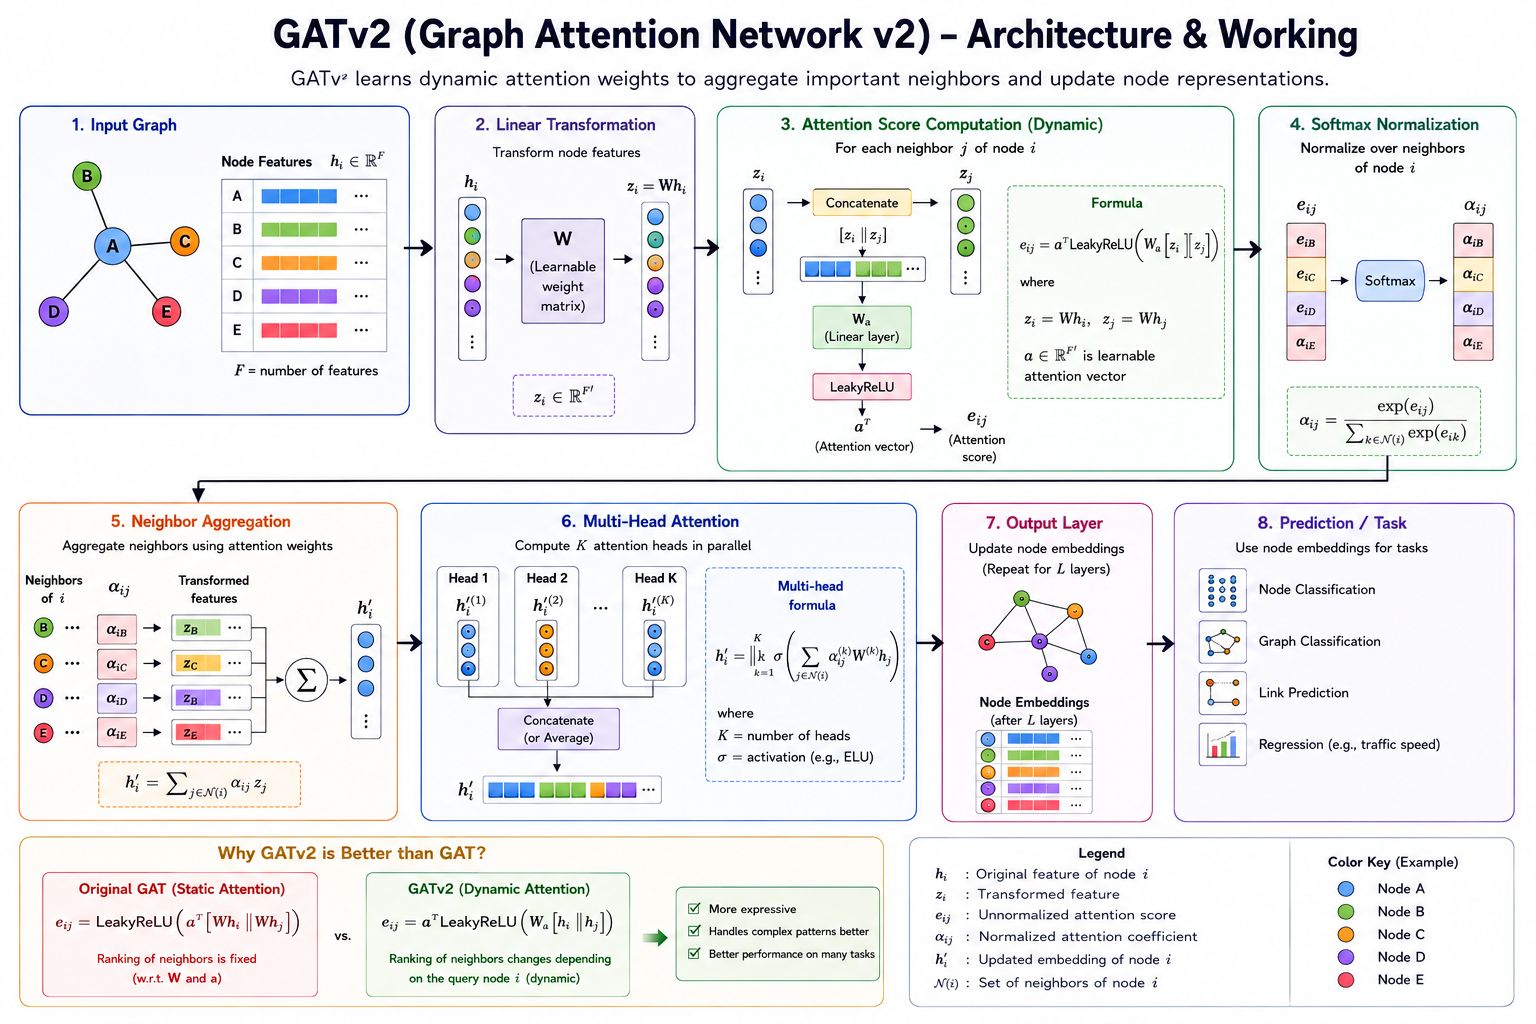
\includegraphics[width=\textwidth]{Figures/GATv2.png}
    \caption{GATv2 Architecture and Working}
    \label{fig:gatv2_architecture}
\end{figure}

The architecture of GATv2 consists of multiple stages including input graph processing, feature transformation, attention computation, normalization, neighbor aggregation, multi-head attention, and prediction generation. Each stage plays a significant role in learning effective graph representations.

\paragraph{Step 1: Input Graph}

The process begins with a graph consisting of nodes, edges, and node feature vectors. Each node contains a feature vector representing its properties.

Mathematically, the node feature vector is represented as:

\[
h_i \in \mathbb{R}^{F}
\]

where:
\begin{itemize}
    \item \(h_i\) represents the feature vector of node \(i\)
    \item \(F\) represents the number of input features
\end{itemize}

In traffic prediction systems, nodes may represent road intersections while edges represent road connectivity. Features may include traffic density, vehicle speed, congestion level, and signal timing information.

\paragraph{Step 2: Linear Transformation}

The input node features are transformed using a learnable weight matrix to extract higher-level representations.

\[
z_i = Wh_i
\]

where:
\begin{itemize}
    \item \(W\) is the learnable weight matrix
    \item \(h_i\) is the original node feature
    \item \(z_i\) is the transformed feature representation
\end{itemize}

This transformation helps the network learn useful combinations of input features and improves feature representation before attention computation.

\paragraph{Step 3: Attention Score Computation}

The attention mechanism is the core component of GATv2. For every connected pair of nodes \((i,j)\), the model computes an attention score representing the importance of neighboring node \(j\) to node \(i\).

The attention mechanism is given by:

\[
e_{ij}=a^{T}\text{LeakyReLU}\left(W[h_i \Vert h_j]\right)
\]

where:
\begin{itemize}
    \item \(h_i\) and \(h_j\) are node feature vectors
    \item \([h_i \Vert h_j]\) represents concatenation
    \item \(W\) is the learnable weight matrix
    \item \(a\) is the learnable attention vector
    \item \(e_{ij}\) is the unnormalized attention score
\end{itemize}

This mechanism dynamically determines the importance of neighboring nodes.

\paragraph{Step 4: Softmax Normalization}

The attention scores are normalized using the softmax function to convert them into probability values.

\[
\alpha_{ij} = \frac{\exp(e_{ij})}{\sum_{k \in \mathcal{N}(i)} \exp(e_{ik})}
\]

where:
\begin{itemize}
    \item \(\alpha_{ij}\) is the normalized attention coefficient
    \item \(\mathcal{N}(i)\) represents the neighboring nodes of node \(i\)
\end{itemize}

This normalization ensures that the attention coefficients sum to 1 and represent the relative importance of neighboring nodes.

\paragraph{Step 5: Neighbor Aggregation}

The neighboring node features are aggregated using weighted summation based on the attention coefficients.

\[
h_i^{\prime} = \sum_{j \in \mathcal{N}(i)} \alpha_{ij}Wh_j
\]

where:
\begin{itemize}
    \item \(h_i^{\prime}\) is the updated node representation
    \item \(\alpha_{ij}\) is the attention coefficient
    \item \(Wh_j\) is the transformed neighboring feature
\end{itemize}

This step allows important neighbors to contribute more significantly to the updated node embedding.

\paragraph{Step 6: Multi-Head Attention}

GATv2 uses multiple attention heads operating in parallel. Each attention head learns different relationships and feature interactions within the graph.

The multi-head attention mechanism is represented as:

\[
h_i^{\prime} =
\mathop{\Vert}_{k=1}^{K}
\sigma
\left(
\sum_{j \in \mathcal{N}(i)}
\alpha_{ij}^{(k)}W^{(k)}h_j
\right)
\]

where:
\begin{itemize}
    \item \(K\) is the number of attention heads
    \item \(\sigma\) is the activation function
    \item \(\Vert\) denotes concatenation
\end{itemize}

Multi-head attention improves learning capability by capturing multiple feature relationships simultaneously.

\paragraph{Step 7: Output Layer and Prediction}

The final node embeddings generated by the attention layers are passed to the output layer for downstream tasks such as:
\begin{itemize}
    \item Node classification
    \item Graph classification
    \item Link prediction
    \item Regression tasks
\end{itemize}

The learned node embeddings contain rich structural and semantic information that helps improve prediction accuracy.

\subsubsection{Advantages of GATv2}

The major advantages of GATv2 are as follows:

\begin{itemize}
    \item Dynamic attention mechanism enables adaptive neighbor importance learning.
    
    \item Improved expressiveness compared to the original GAT architecture.
    
    \item Automatically identifies important neighboring nodes without manual feature engineering.
    
    \item Multi-head attention improves robustness and representation learning.
    
    \item Performs effectively on irregular graph-structured data.
    
    \item Suitable for applications such as traffic prediction, recommendation systems, and autonomous navigation.
\end{itemize}

\subsubsection{Limitations of GATv2}

Despite its advantages, GATv2 also has certain limitations:

\begin{itemize}
    \item Computational complexity increases for large-scale graphs.
    
    \item Requires higher memory consumption due to attention computations.
    
    \item Training time increases with the number of nodes and edges.
    
    \item Deep GATv2 architectures may suffer from over-smoothing problems.
    
    \item Scalability becomes challenging for extremely large graph datasets.
\end{itemize}
\subsubsection{GATv2 vs GAT}

Graph Attention Network v2 (GATv2) was introduced as an improvement over the original Graph Attention Network (GAT) to overcome the limitation of static attention mechanisms. Although both architectures use attention-based aggregation for graph representation learning, GATv2 provides a more expressive and dynamic attention mechanism.

In the original GAT architecture, the ranking of neighboring nodes becomes fixed after the linear transformation step. This limitation reduces the flexibility of the model in learning complex relationships between nodes. The attention mechanism in GAT is given by:

\[
e_{ij} = \text{LeakyReLU}\left(a^{T}[Wh_i \Vert Wh_j]\right)
\]

In GATv2, the order of operations is modified to make the attention mechanism dynamic and more expressive:

\[
e_{ij}=a^{T}\text{LeakyReLU}\left(W[h_i \Vert h_j]\right)
\]

This modification enables the attention scores to depend dynamically on both source and neighboring nodes, allowing the model to learn more meaningful node relationships.

The major differences between GAT and GATv2 are summarized in Table \ref{tab:gat_vs_gatv2}.

\begin{table}[H]
\centering
\caption{Comparison Between GAT and GATv2}
\label{tab:gat_vs_gatv2}
\begin{tabular}{|p{4cm}|p{4.5cm}|p{4.5cm}|}
\hline
\textbf{Feature} & \textbf{GAT} & \textbf{GATv2} \\
\hline
Attention Type & Static Attention & Dynamic Attention \\
\hline
Neighbor Ranking & Fixed after transformation & Changes dynamically based on node context \\
\hline
Expressiveness & Limited & More expressive \\
\hline
Feature Interaction & Moderate & Improved feature interaction learning \\
\hline
Learning Capability & Lower compared to GATv2 & Better representation learning \\
\hline
Performance & Good & Improved performance on many graph tasks \\
\hline
Flexibility & Less flexible & More adaptive and flexible \\
\hline
\end{tabular}
\end{table}

GATv2 is preferred over GAT because it provides a more powerful and adaptive attention mechanism capable of learning complex graph relationships more effectively. The dynamic attention mechanism allows the model to assign different importance values to neighboring nodes depending on the context of the current node. This improves feature aggregation, representation learning, and prediction accuracy.

Due to these advantages, GATv2 is widely preferred in modern graph-based applications such as traffic prediction, autonomous vehicle navigation, recommendation systems, and social network analysis.


\subsection{Long Short-Term Memory (LSTM)}

\subsubsection{Introduction to LSTM}

Shortly after the first Elman-style Recurrent Neural Networks (RNNs) were trained using backpropagation, researchers observed a major limitation in learning long-term dependencies. This problem mainly occurred because of:

\begin{itemize}
    \item Vanishing gradients
    \item Exploding gradients
\end{itemize}

Although gradient clipping could help reduce exploding gradients, handling vanishing gradients required a more advanced solution. To solve this issue, Hochreiter and Schmidhuber introduced the Long Short-Term Memory (LSTM) architecture in 1997.

Unlike standard RNNs, where each recurrent node simply passes information to the next time step, LSTMs introduce a special structure called a memory cell. This memory cell maintains an internal state that allows information to persist over many time steps without vanishing.

The key idea behind LSTM is the ability to:

\begin{itemize}
    \item Remember important information
    \item Forget irrelevant information
    \item Control the flow of information through gates
\end{itemize}

This enables LSTMs to learn long-term sequential dependencies effectively.

\subsubsection{Gated Memory Cell}

Each memory cell is equipped with an internal state and a number of multiplicative gates that determine whether:
\begin{enumerate}
    \item A given input should impact the internal state (the input gate),
    \item The internal state should be flushed to 0 (the forget gate), and
    \item The internal state of a given neuron should be allowed to impact the cell’s output (the output gate).
\end{enumerate}

\subsubsection{Gated Hidden State}

The key distinction between vanilla RNNs and LSTMs is that the latter support gating of the hidden state. This means that we have dedicated mechanisms for when a hidden state should be updated and also for when it should be reset. These mechanisms are learned and they address the concerns listed above. For instance, if the first token is of great importance we will learn not to update the hidden state after the first observation. Likewise, we will learn to skip irrelevant temporary observations. Last, we will learn to reset the latent state whenever needed. We discuss this in detail below.

\subsubsection{Input Gate, Forget Gate, and Output Gate}

The data feeding into the LSTM gates are the input at the current time step and the hidden state of the previous time step, as illustrated in Fig.~10.1.1. Three fully connected layers with sigmoid activation functions compute the values of the input, forget, and output gates. As a result of the sigmoid activation, all values of the three gates are in the range of $(0,1)$.

Additionally, we require an input node, typically computed with a \texttt{tanh} activation function. Intuitively, the input gate determines how much of the input node’s value should be added to the current memory cell internal state. The forget gate determines whether to keep the current value of the memory or flush it. The output gate determines whether the memory cell should influence the output at the current time step.

\begin{figure}[H]
    \centering
    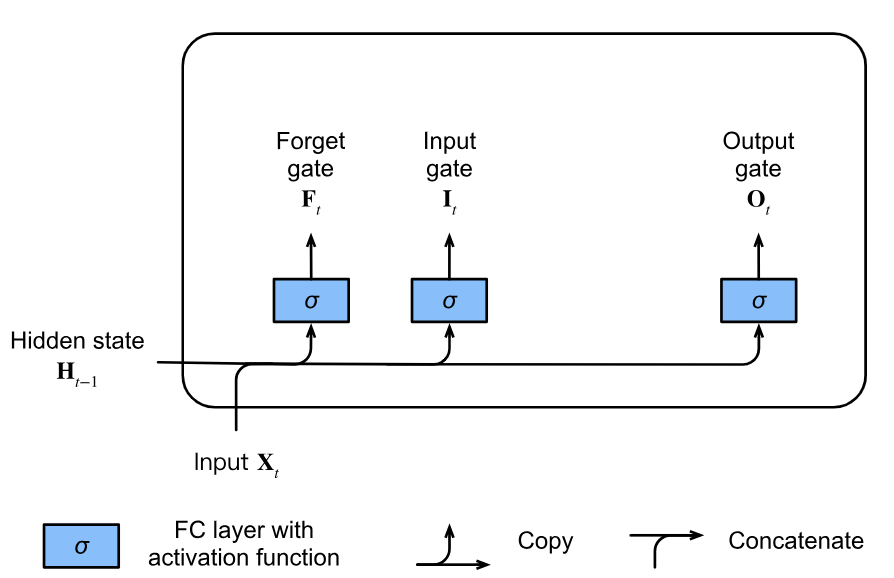
\includegraphics[width=0.7\textwidth]{Figures/LSTM_0}
    \caption{Computing the input gate, the forget gate, and the output gate in an LSTM model}
    \label{fig:lstm_gates}
\end{figure}

Mathematically, suppose that there are $h$ hidden units, the batch size is $n$, and the number of inputs is $d$. Thus, the input is $\mathbf{X}_t \in \mathbb{R}^{n \times d}$ and the hidden state of the previous time step is $\mathbf{H}_{t-1} \in \mathbb{R}^{n \times h}$.

Correspondingly, the gates at time step $t$ are defined as follows: the input gate is $\mathbf{I}_t \in \mathbb{R}^{n \times h}$, the forget gate is $\mathbf{F}_t \in \mathbb{R}^{n \times h}$, and the output gate is $\mathbf{O}_t \in \mathbb{R}^{n \times h}$. They are calculated as follows:

\begin{equation}
\begin{aligned}
\mathbf{I}_t &= \sigma(\mathbf{X}_t \mathbf{W}_{\textrm{xi}} + \mathbf{H}_{t-1} \mathbf{W}_{\textrm{hi}} + \mathbf{b}_{\textrm{i}}),\\
\mathbf{F}_t &= \sigma(\mathbf{X}_t \mathbf{W}_{\textrm{xf}} + \mathbf{H}_{t-1} \mathbf{W}_{\textrm{hf}} + \mathbf{b}_{\textrm{f}}),\\
\mathbf{O}_t &= \sigma(\mathbf{X}_t \mathbf{W}_{\textrm{xo}} + \mathbf{H}_{t-1} \mathbf{W}_{\textrm{ho}} + \mathbf{b}_{\textrm{o}})
\end{aligned}
\end{equation}

where $\mathbf{W}_{\textrm{xi}}, \mathbf{W}_{\textrm{xf}}, \mathbf{W}_{\textrm{xo}} \in \mathbb{R}^{d \times h}$ and $\mathbf{W}_{\textrm{hi}}, \mathbf{W}_{\textrm{hf}}, \mathbf{W}_{\textrm{ho}} \in \mathbb{R}^{h \times h}$ are weight parameters and $\mathbf{b}_{\textrm{i}}, \mathbf{b}_{\textrm{f}}, \mathbf{b}_{\textrm{o}} \in \mathbb{R}^{1 \times h}$ are bias parameters.

Note that broadcasting is triggered during the summation. We use sigmoid functions to map the input values to the interval $(0,1)$.

\subsubsection{Input Node}

Next we design the memory cell. Since we have not specified the action of the various gates yet, we first introduce the input node $\tilde{\mathbf{C}}_t \in \mathbb{R}^{n \times h}$. Its computation is similar to that of the three gates described above, but uses a \texttt{tanh} function with a value range for $(-1,1)$ as the activation function. This leads to the following equation at time step $t$:

\begin{equation}
\tilde{\mathbf{C}}_t = \textrm{tanh}(\mathbf{X}_t \mathbf{W}_{\textrm{xc}} + \mathbf{H}_{t-1} \mathbf{W}_{\textrm{hc}} + \mathbf{b}_{\textrm{c}})
\end{equation}

where $\mathbf{W}_{\textrm{xc}} \in \mathbb{R}^{d \times h}$ and $\mathbf{W}_{\textrm{hc}} \in \mathbb{R}^{h \times h}$ are weight parameters and $\mathbf{b}_{\textrm{c}} \in \mathbb{R}^{1 \times h}$ is a bias parameter.

A quick illustration of the input node is shown in Fig.~10.1.2.

\begin{figure}[H]
    \centering
    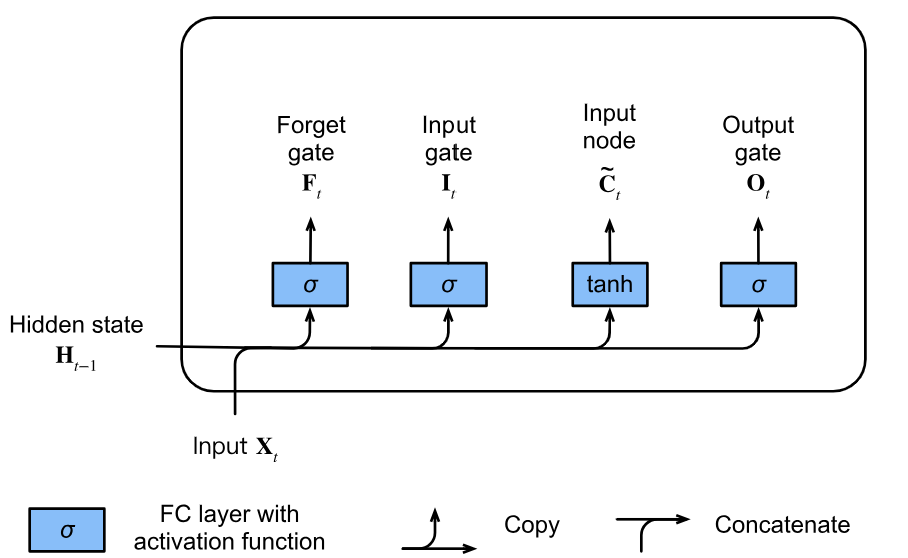
\includegraphics[width=0.7\textwidth]{Figures/LSTM_1}
    \caption{Computing the input node in an LSTM model}
    \label{fig:lstm_input_node}
\end{figure}

\subsubsection{Memory Cell Internal State}

In LSTMs, the input gate $\mathbf{I}_t$ governs how much we take new data into account via $\tilde{\mathbf{C}}_t$ and the forget gate $\mathbf{F}_t$ addresses how much of the old cell internal state $\mathbf{C}_{t-1} \in \mathbb{R}^{n \times h}$ we retain. Using the Hadamard (elementwise) product operator $\odot$ we arrive at the following update equation:

\begin{equation}
\mathbf{C}_t = \mathbf{F}_t \odot \mathbf{C}_{t-1} + \mathbf{I}_t \odot \tilde{\mathbf{C}}_t
\end{equation}

If the forget gate is always 1 and the input gate is always 0, the memory cell internal state $\mathbf{C}_{t-1}$ will remain constant forever, passing unchanged to each subsequent time step. However, input gates and forget gates give the model the flexibility of being able to learn when to keep this value unchanged and when to perturb it in response to subsequent inputs.

In practice, this design alleviates the vanishing gradient problem, resulting in models that are much easier to train, especially when facing datasets with long sequence lengths.

We thus arrive at the flow diagram in Fig.~10.1.3.

\begin{figure}[H]
    \centering
    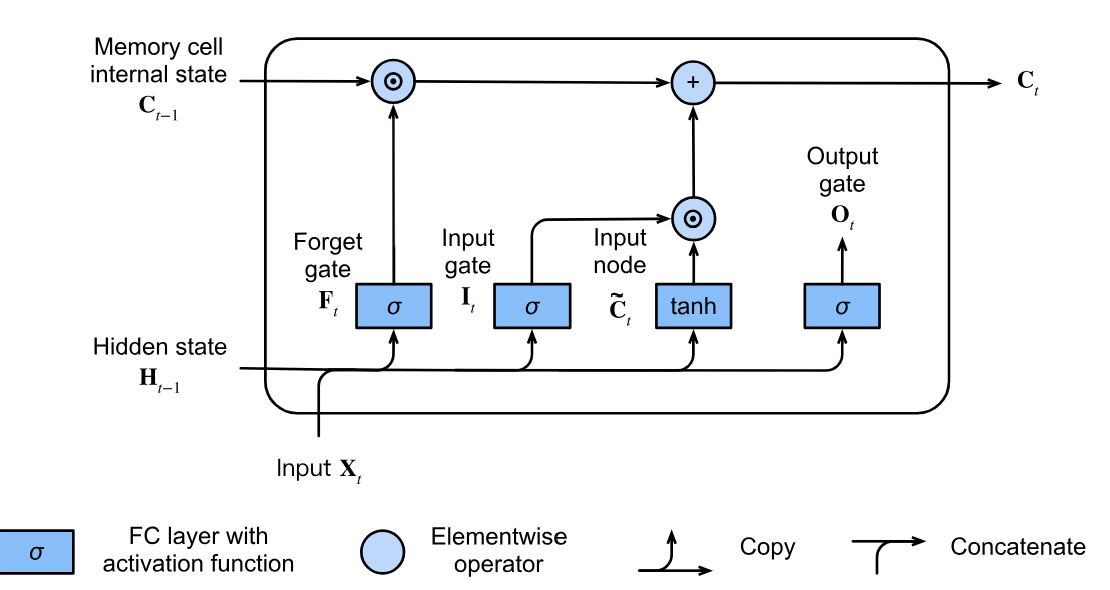
\includegraphics[width=0.7\textwidth]{Figures/LSTM_2}
    \caption{Computing the memory cell internal state in an LSTM model}
    \label{fig:lstm_memory_cell}
\end{figure}

\subsubsection{Hidden State}

Last, we need to define how to compute the output of the memory cell, i.e., the hidden state $\mathbf{H}_t \in \mathbb{R}^{n \times h}$, as seen by other layers. This is where the output gate comes into play.

In LSTMs, we first apply \texttt{tanh} to the memory cell internal state and then apply another point-wise multiplication, this time with the output gate. This ensures that the values of $\mathbf{H}_t$ are always in the interval $(-1,1)$:

\begin{equation}
\mathbf{H}_t = \mathbf{O}_t \odot \tanh(\mathbf{C}_t)
\end{equation}

Whenever the output gate is close to 1, we allow the memory cell internal state to impact the subsequent layers uninhibited, whereas for output gate values close to 0, we prevent the current memory from impacting other layers of the network at the current time step.

Note that a memory cell can accrue information across many time steps without impacting the rest of the network (as long as the output gate takes values close to 0), and then suddenly impact the network at a subsequent time step as soon as the output gate flips from values close to 0 to values close to 1.

Fig.~10.1.4 has a graphical illustration of the data flow.

\begin{figure}[H]
    \centering
    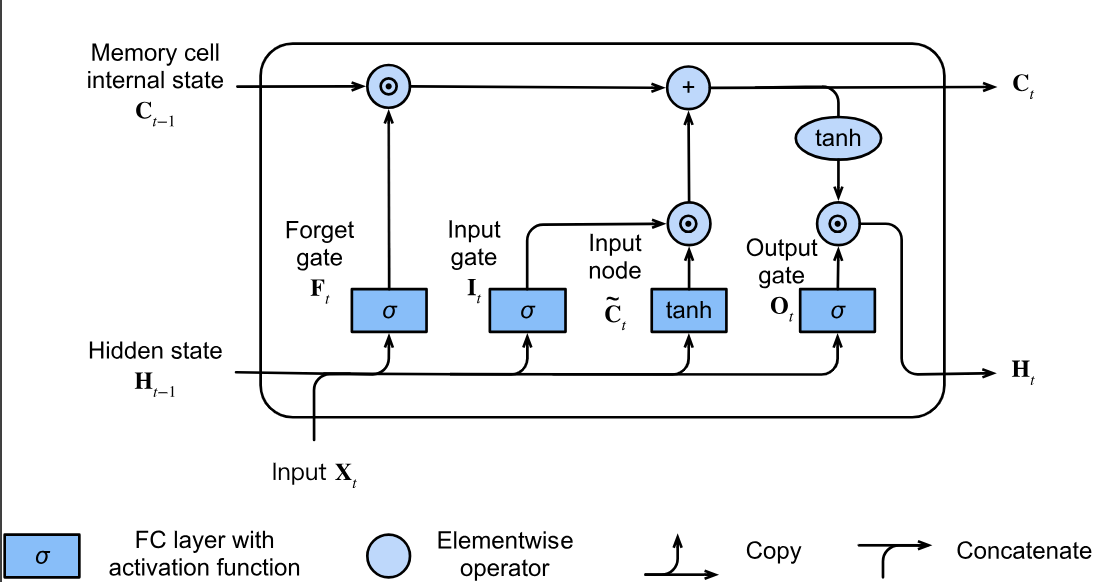
\includegraphics[width=0.7\textwidth]{Figures/LSTM_3}
    \caption{Computing the hidden state in an LSTM model}
    \label{fig:lstm_hidden_state}
\end{figure}

\subsubsection{Advantages of LSTM}

The major advantages of LSTM are as follows:

\begin{itemize}
    \item LSTM effectively solves the vanishing gradient problem faced by traditional Recurrent Neural Networks (RNNs).
    
    \item It can learn long-term dependencies and preserve information over extended sequence lengths.
    
    \item The gating mechanism enables selective memory retention and controlled information flow.
    
    \item LSTM performs well on sequential and time-series data.
    
    \item It is highly effective in applications such as natural language processing, speech recognition, machine translation, traffic prediction, and stock market forecasting.
    
    \item The memory cell architecture allows important information to persist across multiple time steps.
    
    \item LSTM networks are more stable and easier to train compared to vanilla RNNs.
\end{itemize}

\subsubsection{Limitations of LSTM}

Despite its advantages, LSTM also has certain limitations:

\begin{itemize}
    \item LSTM networks are computationally expensive due to the presence of multiple gates and memory cells.
    
    \item Training LSTM models requires high computational power and longer training time.
    
    \item The architecture is more complex compared to traditional RNNs.
    
    \item LSTMs require a large amount of training data for better generalization.
    
    \item They may suffer from overfitting when trained on small datasets.
    
    \item Parallel processing is difficult because sequential data must be processed step-by-step.
    
    \item For extremely long sequences, performance may still degrade despite improved memory retention.
\end{itemize}

\textit{Source: Adapted from ``Dive into Deep Learning,Long Short-Term Memory \href{https://d2l.ai/chapter_recurrent-modern/lstm.html?utm_source=chatgpt.com}{(LSTM)}."}

\vspace{0.3cm}





%========================================================
\section{User Interface}
%========================================================

Modern financial monitoring platforms increasingly rely on scalable web application technologies to support real-time transaction analysis, fraud monitoring, and interactive visualization of financial activities. The rapid growth of digital banking and online financial services has significantly increased the demand for responsive, secure, and data-driven monitoring systems capable of handling large volumes of transactional information efficiently. Consequently, modern Anti-Money Laundering systems employ component-based web architectures and client-server communication models to provide efficient user interaction and real-time analytical capabilities.

Advanced frontend frameworks and backend service architectures play a critical role in enabling modular application development, dynamic rendering, secure authentication, and seamless integration with fraud detection engines. Such technologies support the visualization of suspicious transactional activities, alert generation, role-based access control, and automated compliance workflows within financial institutions. The integration of scalable user interface technologies with intelligent analytical systems further enhances operational efficiency and supports real-time financial crime investigation processes.

%========================================================
\subsection[Modern Web Application Frameworks]{\textbf{Modern Web Application Frameworks}}
%========================================================

Modern web application frameworks provide the architectural foundation required for developing scalable, responsive, and interactive software systems. Traditional web applications primarily relied on static page rendering and tightly coupled server-side architectures, which limited dynamic user interaction and real-time data processing capabilities. In contrast, modern frameworks adopt component-based and asynchronous rendering approaches that improve application scalability, maintainability, and user experience within large-scale distributed systems.

Frontend frameworks such as React.js enable the development of reusable and modular user interface components capable of dynamically updating application states without requiring complete page reloads. Such frameworks employ virtual Document Object Model (DOM) mechanisms and state-driven rendering principles to efficiently manage user interactions and real-time data visualization. This architectural approach significantly improves responsiveness and enables scalable dashboard development for data-intensive applications such as financial monitoring systems.

Server-side rendering and hybrid rendering frameworks such as Next.js further enhance modern web application performance by combining client-side interactivity with optimized server-side content delivery. These frameworks support efficient routing, dynamic data fetching, and improved application scalability while reducing rendering overhead for large-scale systems. Consequently, modern web application frameworks have become an essential foundation for building secure, scalable, and real-time financial monitoring platforms.

%========================================================
\subsection[Component Lifecycle and Reactivity]{\textbf{Component Lifecycle and Reactivity}}
%========================================================

Modern web application frameworks employ reactive rendering mechanisms to dynamically synchronize the user interface with application data and user interactions. In component-based architectures such as React and Next.js, the user interface continuously responds to changes in application state, backend responses, and client-side events. This reactive behavior enables efficient rendering of dynamic content while improving scalability, responsiveness, and maintainability within large-scale financial monitoring systems.

The component lifecycle in modern React and Next.js applications generally follows a sequence of rendering, interaction, updating, and cleanup stages. These stages collectively manage how components are initialized, rendered, updated, and removed during application execution. The overall lifecycle flow can be summarized as follows:

\begin{itemize}

\item \textbf{Server-Side Rendering:}  
Initially, application components are rendered within the server environment where data fetching and content generation are performed before transmitting the rendered output to the client browser. This approach improves initial loading performance and reduces unnecessary client-side computational overhead.

\item \textbf{Hydration and Client Initialization:}  
After the rendered HTML content reaches the client browser, React hydrates the interface by attaching event listeners and enabling interactive functionalities within client-side components. During this stage, local states, dynamic properties, and asynchronous operations are initialized for user interaction.

\item \textbf{Reactive State Updates:}  
As users interact with the application, component states and properties continuously change according to system events and backend responses. React employs Virtual DOM reconciliation mechanisms to compare interface changes and selectively update only the affected components instead of re-rendering the complete application interface.

\item \textbf{Re-rendering and Synchronization:}  
Whenever state transitions occur, the framework dynamically re-renders the modified components and synchronizes the updated data with the user interface. This reactive rendering process enables real-time visualization of financial transactions, fraud alerts, and monitoring analytics within Anti-Money Laundering dashboards.

\item \textbf{Unmounting and Resource Cleanup:}  
When components are removed from the active interface, allocated resources, subscriptions, and temporary states are released to maintain application stability and efficient memory utilization.

\end{itemize}

Such lifecycle management principles are essential in modern financial monitoring platforms where continuous transactional updates, alert generation, and real-time analytical visualization must be processed efficiently while ensuring scalable and responsive user interaction.



%========================================================
\subsection[Data Visualization and Monitoring Dashboards]{\textbf{Data Visualization and Monitoring Dashboards}}
%========================================================

Understanding the theoretical aspects of data visualization is important for analyzing large volumes of financial transactions and interpreting suspicious transactional behavior within real-time monitoring systems. Visualization of analytical outputs enables financial institutions and compliance analysts to identify fraud patterns, transaction anomalies, risk distributions, and suspicious entity relationships more efficiently when compared with conventional tabular analysis methods. Interactive monitoring dashboards further improve situational awareness by enabling continuous observation of fraud alerts, transaction flows, and compliance activities without interrupting real-time analytical processes.

This work conceptualizes financial monitoring and fraud visualization through a web-based dashboard architecture developed using modern frontend technologies and analytical visualization frameworks:

\begin{itemize}

\item \textbf{Nextjs} is employed as the frontend framework for developing responsive and modular user interface components capable of supporting scalable financial monitoring applications.

\item \textbf{Recharts} is utilized for visualizing transactional analytics, fraud classifications, risk score distributions, and temporal financial trends through interactive line graphs, bar charts, pie charts, and statistical dashboards.

\item \textbf{Role-based dashboard interfaces} enable controlled access to monitoring functionalities, fraud investigation workflows, Suspicious Transaction Report (STR) generation, and real-time alert visualization according to user privileges and institutional responsibilities.

\item \textbf{Interactive analytical panels} support continuous monitoring of suspicious activities, transaction histories, and fraud prediction results generated by intelligent detection systems operating within the platform.

\end{itemize}

Modern visualization systems additionally support notification mechanisms, analytical filtering, and export functionalities that assist investigators and compliance officers in conducting financial analysis and generating compliance reports for further examination. The detailed implementation and integration of these visualization technologies within the proposed TBML detection framework are discussed further in the system implementation chapter.


\section*{Summary}

In this chapter, the theoretical foundations required for understanding the proposed Trade-Based Money Laundering detection framework were presented. The chapter began with an introduction to Trade-Based Money Laundering mechanisms and common laundering techniques, establishing the financial and transactional context in which illicit fund movement occurs within international trade ecosystems.

The chapter further explored the challenges associated with detecting suspicious trade activities using conventional Anti-Money Laundering approaches. Concepts related to graph-based financial modeling, heterogeneous graph representation, Graph Neural Networks, Graph Attention mechanisms, and federated learning were discussed to provide the analytical and computational foundation required for intelligent and privacy-preserving fraud detection systems.

Finally, the chapter introduced the concepts associated with modern financial monitoring interfaces, reactive web architectures, and real-time data visualization systems used for fraud analytics and compliance monitoring. The theoretical concepts discussed throughout this chapter provide the foundation for understanding the system architecture, implementation methodologies, and analytical workflows presented in the subsequent chapters.